
\begin{frame}
  \frametitle{Dynamic traffic assignment at Merges}
  \begin{columns}
    \begin{column}{0.5\textwidth}
      Let consider the case: 
      \begin{equation*}
        \begin{aligned}
        \onslide<4->{&\underset{f_i}{\max}& &\sum f_i\\}
        \onslide<1->{&\text{s.t} & & f_1 \leq D_1  \\}
        \onslide<2->{& & & f_2 \leq D_2\\}
        \onslide<3->{& & & f_1 + f_2 \leq S_3}
        \end{aligned}
      \end{equation*}
      \uncover<4-:>{
      \begin{block}{Solution}
        In general the dynamic traffic assingment problem has multiple values \(f_1,f_2\) that may satisfy the problem constraints.
      \end{block}
      }
    \end{column}
    \begin{column}{0.5\textwidth}
      \begin{figure}
        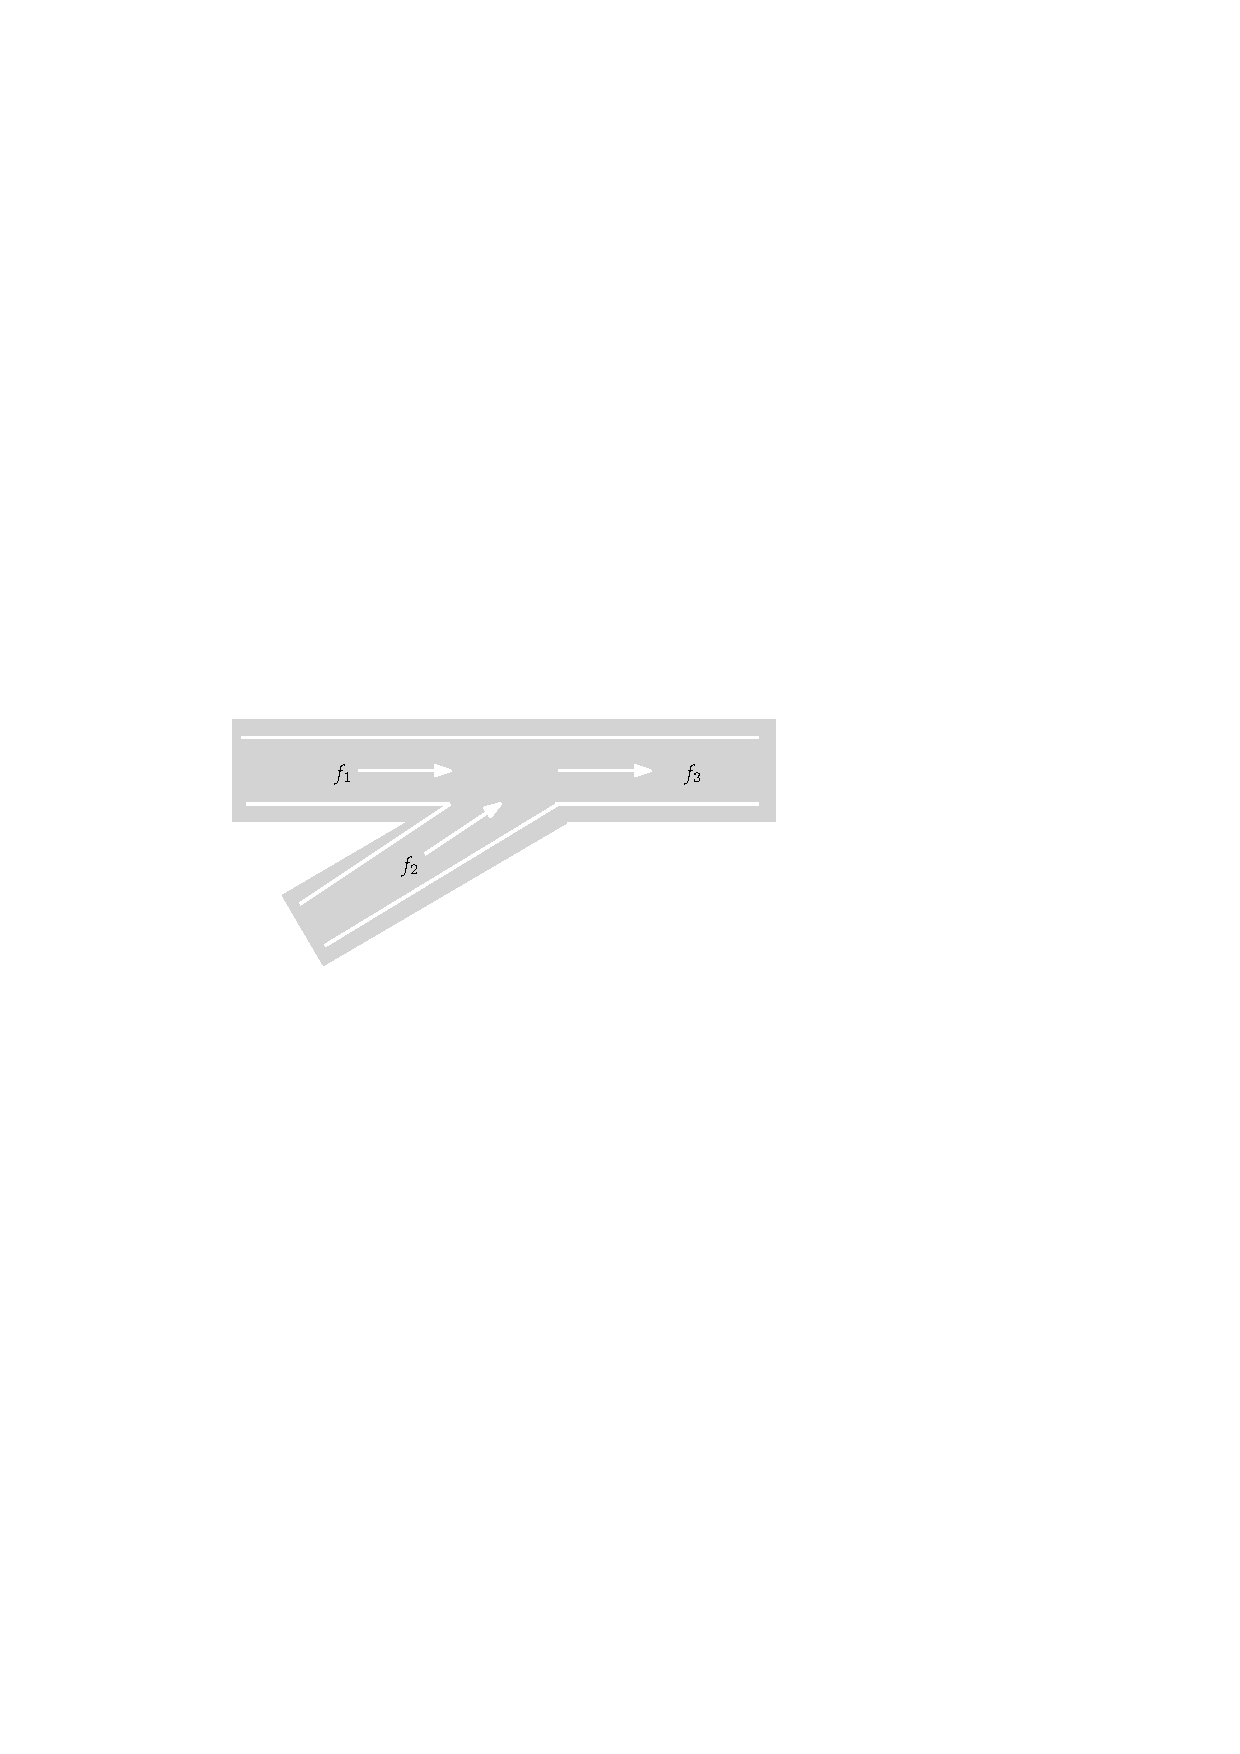
\includegraphics[width=0.8\linewidth]{fig_23b_merge.pdf}
      \end{figure}
      \only<1|handout:0>{
        \begin{figure}
          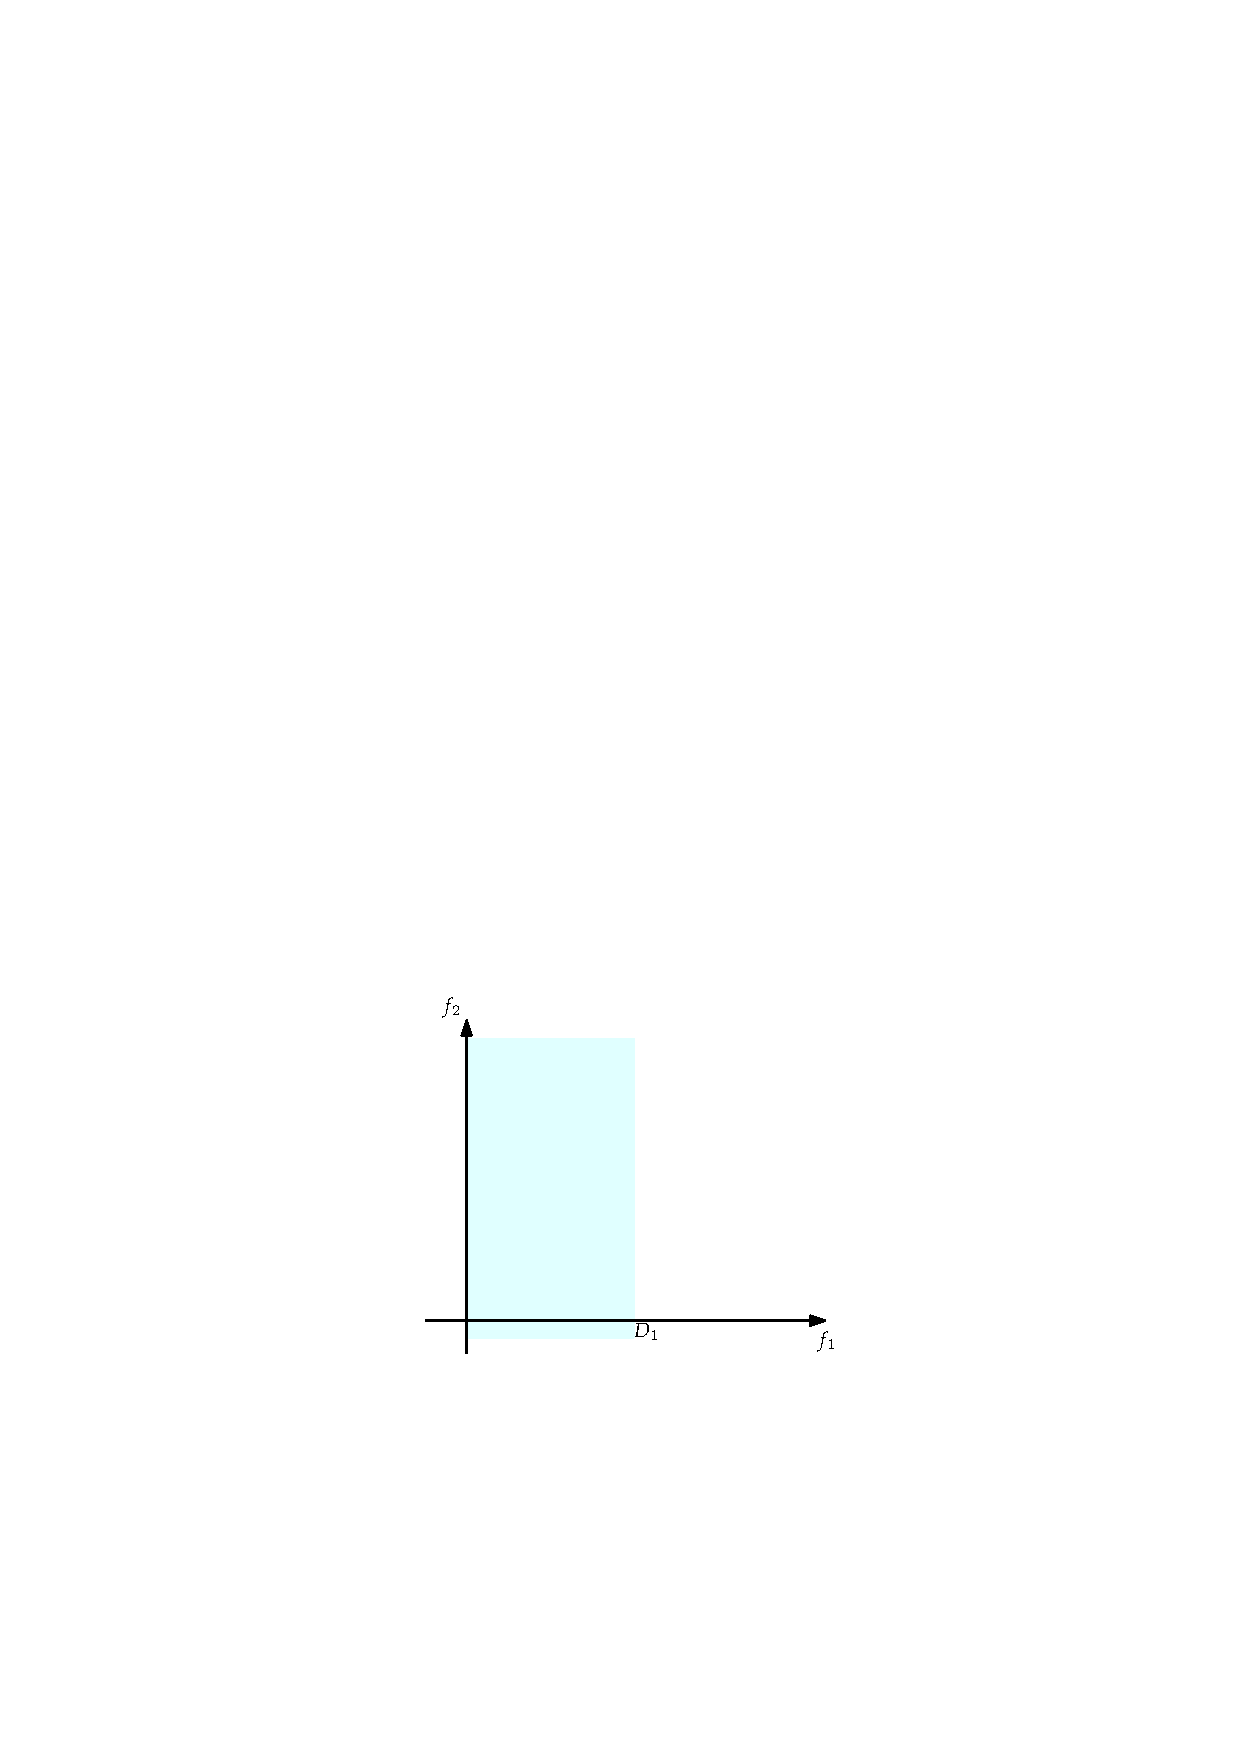
\includegraphics[width=0.8\linewidth]{fig_24a_diagram_merge}
        \end{figure}
      }
      \only<2|handout:0>{
        \begin{figure}
          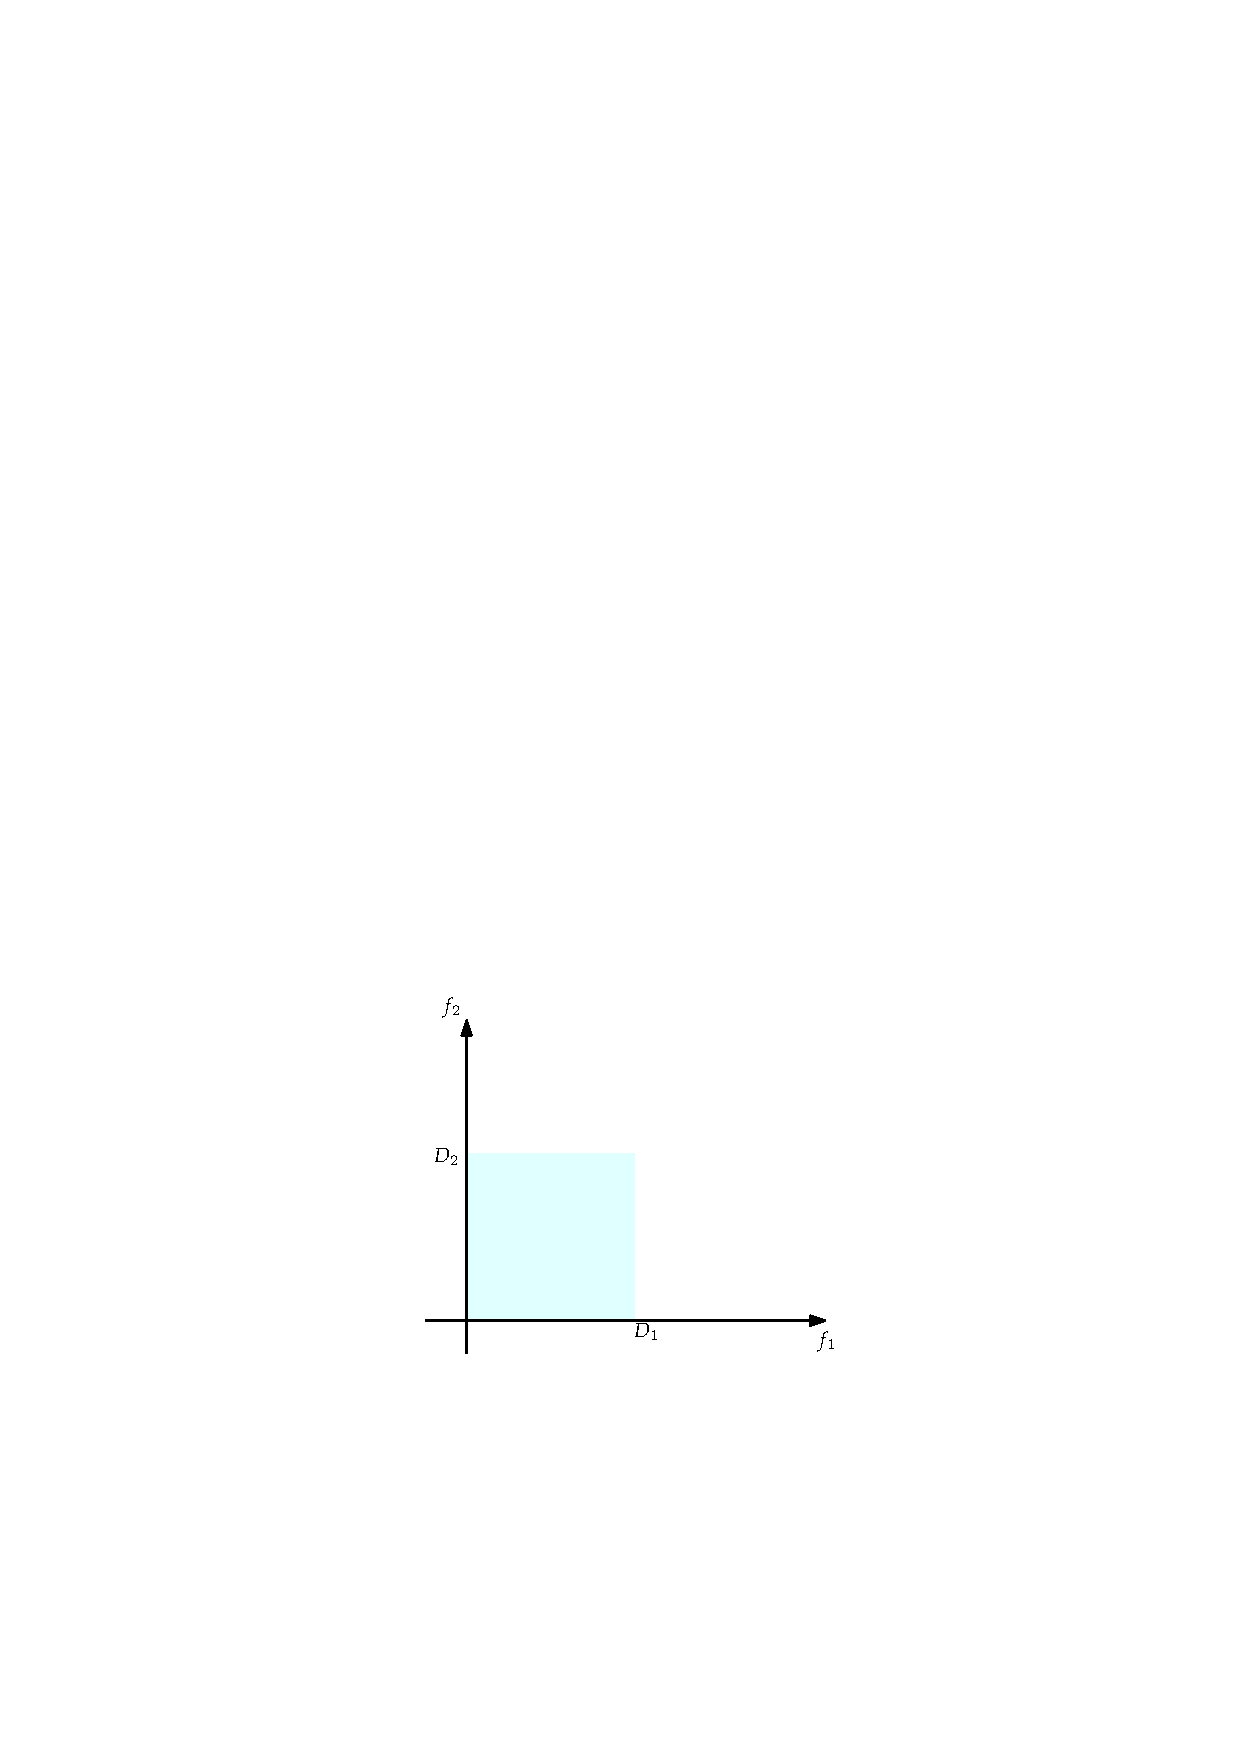
\includegraphics[width=0.8\linewidth]{fig_24b_diagram_merge}
        \end{figure}
      }
      \only<3|handout:0>{
        \begin{figure}
          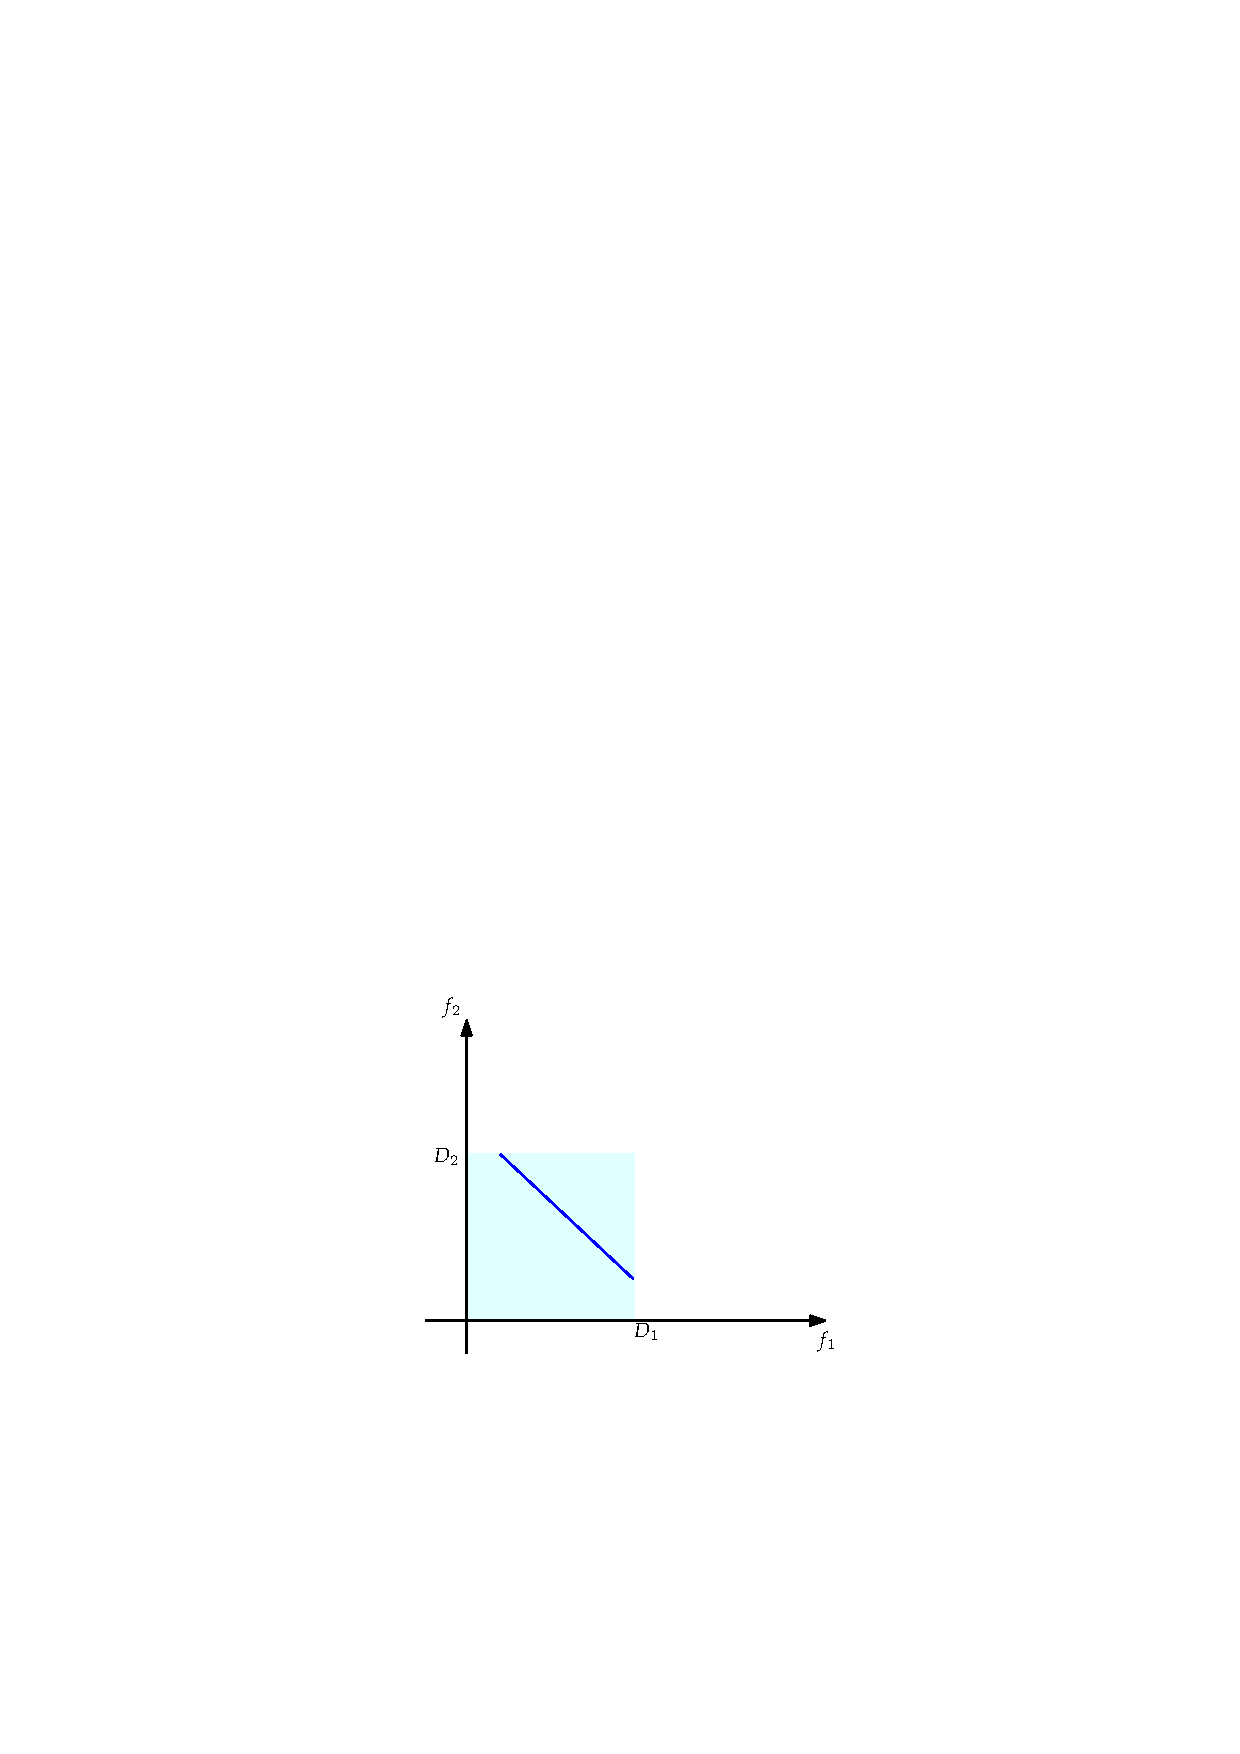
\includegraphics[width=0.8\linewidth]{fig_24c_diagram_merge}
        \end{figure}
      }
      \only<4|handout:1>{
        \begin{figure}
          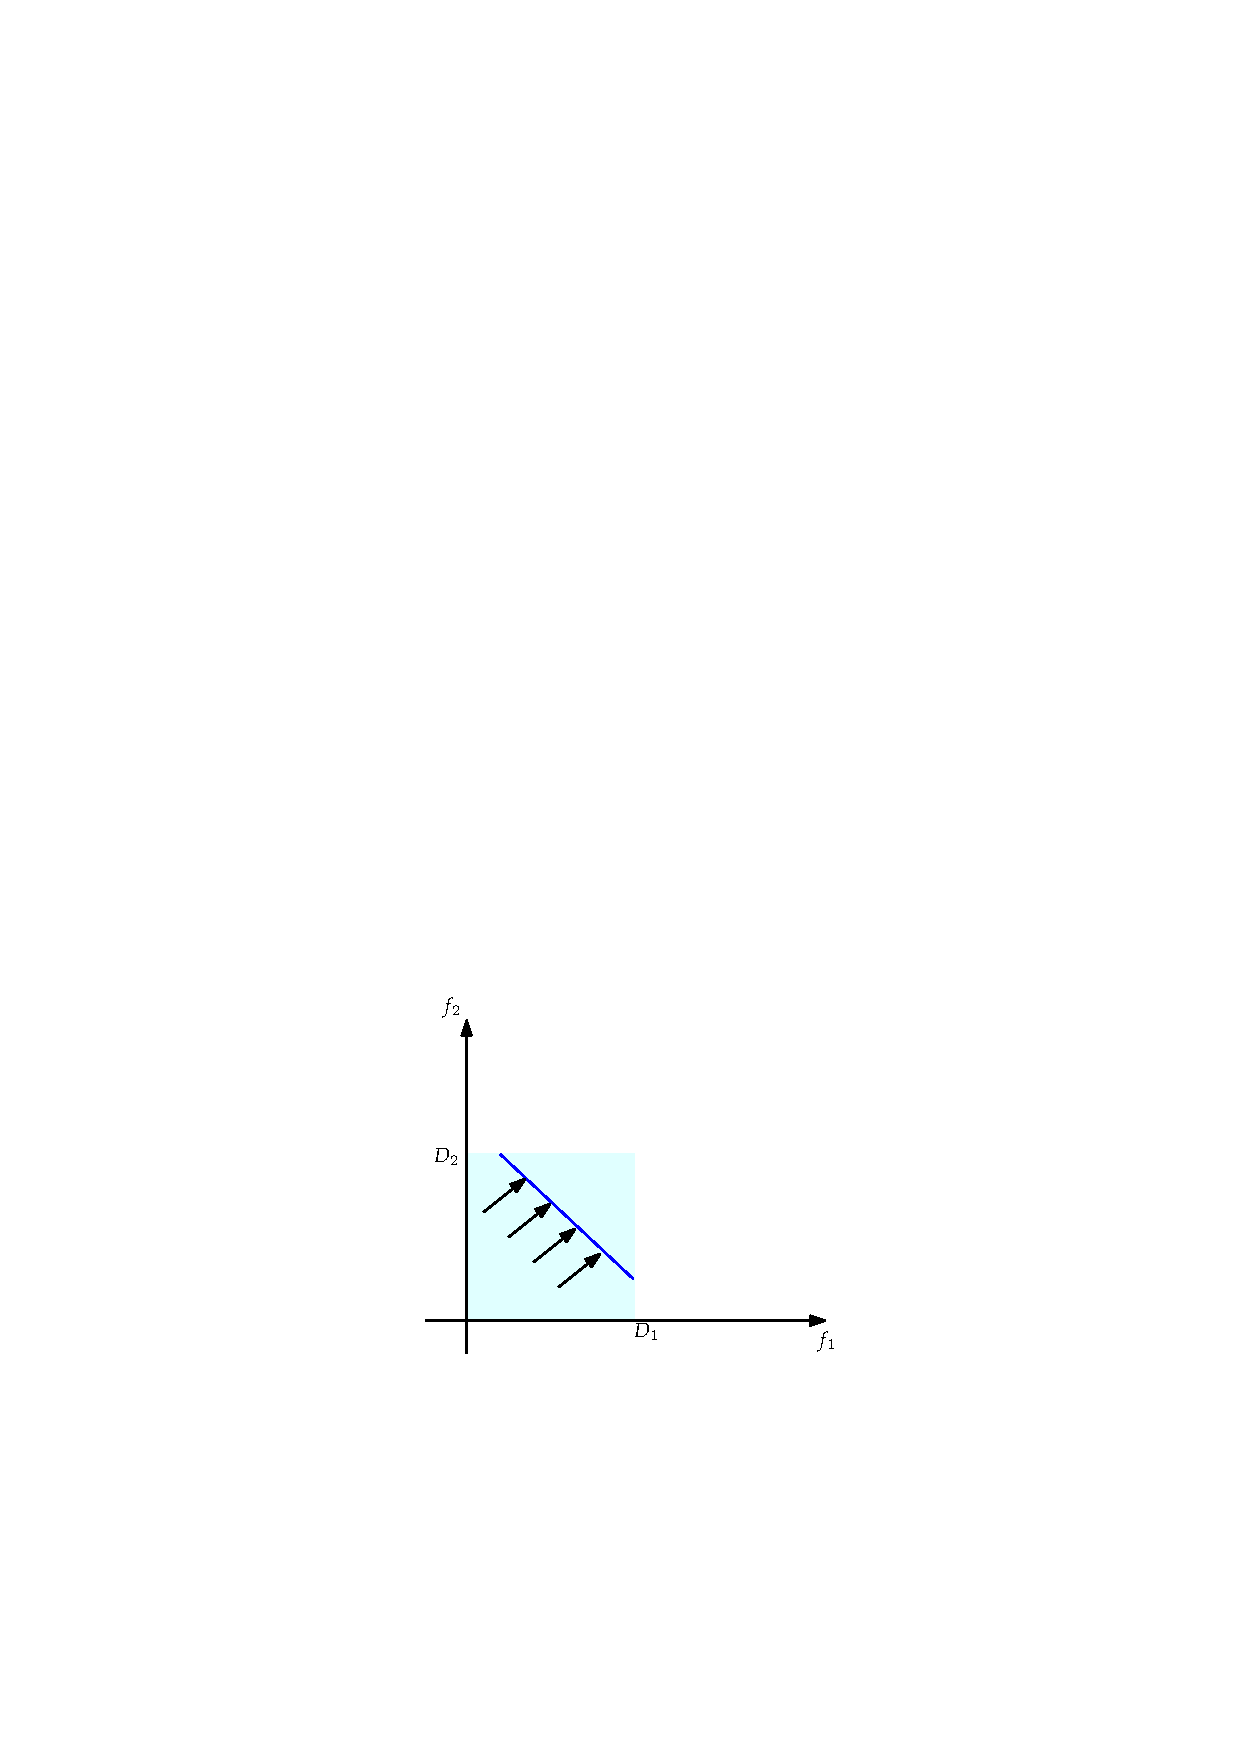
\includegraphics[width=0.8\linewidth]{fig_24d_diagram_merge}
        \end{figure}
      }
    \end{column}
  \end{columns}    
\end{frame}